\documentclass{article}
\usepackage{graphicx} % Required for inserting images
\usepackage{amsmath}
\usepackage{mathtools}
\usepackage{hyperref}
\usepackage{geometry}
\usepackage{tikz}
\usetikzlibrary{angles, quotes}
\usepackage{float}
\geometry{margin=1in}

\newcommand{\norm}[2][]{\left\lVert#2\right\rVert_{#1}}

\title{AI Manifesto: Appreciation of Mathematics Underlying Machine Learning Concepts}

\author{Batuhan Karaca}

\numberwithin{equation}{subsection}
\begin{document}

\maketitle
\tableofcontents
\section{Introduction}
\subsection{TLDR But Binding}
This book aims to give intuition for some machine learning concepts that I thought of significance. I started writing it simply because of the fact that I was bored of reading TLDR textbooks without understanding anything at all. That is why, I tried to give information as concise and as clear as possible. This compound thingy is solely my research and notetaking work piled up over years. 

I am not claiming to have 100\% accurate statements, though have I not seen any conflictions between my findings and the publications. I do not think any theory is perfect as well. They are good only because they just work in practice. Furthermore, I am not claiming this book to be a textbook material on its own. I only wanted to share (hopefully) helpful information for deep understanding of the objects using math, as every scientific finding has a mathematical background in my opinion. Nevertheless, you will see some beliefs of my own as I could not come up with a clear answer (encountering conflicting statements in publications to check thereafter), so I warped it with my thoughts (science huh). For example, the fact that dependence is a superset of correlation in part~\ref{cor_dep} is such a gibberish. However, every other piece starts to fit nicely on each other with this statement (mutual coherency for now). I hope you will come up with your own brilliant ideas utilizing this knowledge and sharing them for all. Public science and open source forever!
\subsection{Useful Part}
It is not mandatory, but recommended to have basic knowledge in linear algebra and probability theory and some familiarity with the concepts (e.g. through courses). 
\subsubsection{Followed Conventions}
Unless stated otherwise, these math notations apply. 
\begin{itemize}
    \item Capital letters represent matrices (or hypermatrices in general) and random variables.
    \item Lowercase symbols denote vectors and scalars.
    \item In some contexts, $0$ and $1$ may indicate a vector or matrix only composed of these scalars.
    \item Vectors are column vectors by default.
    \item Row vectors are denoted as their transpose with a superscript capital $T$ (i.e. $a^T$).
    \item Scalar (or a row/column vector) of a matrix is denoted with corresponding lowercase symbol.
    \item Pre-superscript on a symbol of a matrix denotes the shape of the matrix (i.e. $\prescript{M\times N}{}{A}$ is a matrix $A$ with shape $M\times N$).
    \item Subscript on a lowercase variable symbol (i.e. $a_{ijk...}$) denotes the index of that variable in its corresponding matrix with capital letter. Furthermore, colon between indices indicates the ordered array (vector/matrix etc.) of variables whose indices are bounded between upper and lower bounds ordered (i.e. $a^T_{i:j} = [a^T_i, a^T_{i+1}, ..., a^T_{j-1}]$)
    \item Subscript of an integral or sum symbol denoting a variable (i.e. $\sum_X$, $\int_X$) indicates that the operation spans the entire domain of that variable (i.e. $X$).
    \item Subscript of an expected value symbol (i.e. $E_{p(X)}$) denotes the probability weight of the random variable given in its formula (i.e. $p(X)$).
    \item Aggregation operators such as $\min$ support indexing (i.e. $\min_kx_k = x_{\arg_k\min x_k}$)
\end{itemize}
\section{Linear Algebra Used In Learning and Optimization}
\subsection{Definitions}
\subsubsection{P-Norm}
\begin{align}
    \norm[p]{a} &= (\sum_i a_i^p)^{\frac{1}{p}} &\\
    \norm[1]{a} & & \text{(Manhattan norm)} \label{man_norm}\\
    \norm[2]{a} &= \norm[]{a} & \text{(Euclidean norm)} \label{euc_norm}
\end{align}
\subsection{Proof of Cosine Law}
\begin{figure}[H]
    \centering
    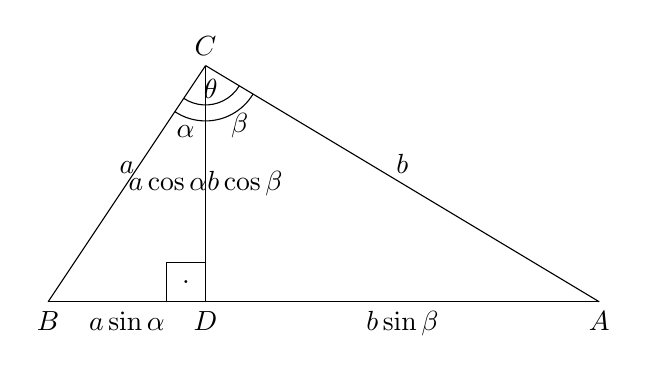
\begin{tikzpicture}
        \coordinate[label=below:$A$] (a) at (7,0); 
        \coordinate[label=below:$B$] (b) at (0,0); 
        \coordinate[label=above:$C$] (c) at (2,3); 
        \coordinate[label=below:$D$] (d) at (2,0); 
        \draw (b) -- (d) node[midway,anchor=north]{$a
        \sin\alpha$};
        \draw (d) -- (a) node[midway,anchor=north]{$b
        \sin \beta$};
        \draw (b) -- (c) node[midway,anchor=south]{$a$};
        \draw (c) -- (a) node[midway,anchor=south]{$b$};
        \draw (c) -- (d) node[midway,anchor=center]{$a \cos \alpha b \cos\beta$};
        \pic[draw, "$\alpha$", angle eccentricity=1.25, angle radius=20] {angle = b--c--d};
        \pic[draw, "$\beta$", angle eccentricity=1.25, angle radius=20] {angle = d--c--a};
        \pic[draw, "$\theta$"] {angle = b--c--a};
        \pic[draw, "$.$", angle eccentricity=.5] {right angle = c--d--b};
        \end{tikzpicture}
    \caption{}
    \label{fig:cos_law_tri}
\end{figure}
Figure~\ref{fig:cos_law_tri} shows a triangle with rules below
\begin{align}
    |BC| &= a \\
    |AC| &= b \\
    |BD| &= a\sin\alpha \\   
    |AD| &= b\sin\beta \\
    |CD| &= a\cos\alpha = b\cos\beta\\
    |AB| &= |BD|+|AD|\\
    |CD| \bot |AB|\\
    \angle{BCD} &= \alpha\\
    \angle{DCA} &= \beta \\
    \angle{BCA} &= \theta = \angle{BCD} + \angle{DCA}
\end{align}


\begin{align}
    c &= a\sin\alpha + b\sin \beta\\
    c^2 &= a^2\sin^2 \alpha + b^2\sin^2 \beta + 2ab\sin\alpha\sin \beta\\
     &= a^2\sin^2 \alpha + b^2\sin^2 \beta + 2ab[\cos \alpha\cos\beta - \cos(\alpha +\beta)]\ \text{by trigonometric identities}\\
     &= a^2\sin^2 \alpha + b^2\sin^2 \beta + ab\cos \alpha\cos\beta + ab\cos \alpha\cos\beta - 2ab\cos(\alpha +\beta)\\
     &= a^2\sin^2 \alpha + b^2\sin^2 \beta + a^2\cos^2 \alpha + b^2\cos^2 \beta - 2ab\cos(\alpha +\beta)\\
     &= a^2(\sin\alpha^2 + \cos \alpha^2) + b^2(\sin^2 \beta + \cos^2 \beta) - 2ab\cos(\alpha +\beta)\\
     &= a^2 + b^2 - 2ab\cos(\alpha +\beta)\\
     &= a^2 + b^2 - 2ab\cos \theta \label{cos_law}
\end{align}
\subsection{Relation Between Dot Product and Cosine}
Assume
\begin{equation}
    c = a-b
\end{equation}
such that $a, b$ and $c$ are vectors. We define an operation (dot product) on vectors which has following properties

\begin{itemize}
    \item commutativity (i.e. $a^Tb = b^Ta$)
    \item distributivity (i.e. $a^T(b+c) = a^Tb+a^Tc)$)
    \item dot product of a vector with itself is equivalent to squared Euclidean norm (length) (i.e. $a^Ta = \norm{a}^2$)
\end{itemize}
and many other properties of the scalar multiplication we know of (In fact, the well known dot product formula $a^Tb = \sum_i a_i b_i$ satisfies all of these properties).
These properties in mind we find
\begin{align}
    c^2 &= (a-b)^T(a-b)\\
    &= a^Ta +b^Tb - 2a^Tb\\
\end{align}
Using~\ref{cos_law} (note that the values shown there are scalar lengths)
\begin{align}
    a^Ta +b^Tb - 2a^Tb &= \norm{a}^2 + \norm{b}^2 - 2\norm{a}\norm{b}\cos \theta\\
    a^Tb &= \norm{a}\norm{b}\cos \theta
\end{align}
Now for a given point $p$ and normal vector $a$, every point $x$ making $a$ and $(x-p)$ perpendicular to each other ($\theta = \frac{\pi}{2}$) 
\begin{align}
    a^T(x-p) &= 0\\
    a^Tx-a^Tp &= 0\\
    a^Tx+b &= 0
\end{align}
indeed spans a hyperplane. Notice $b = -a^Tp$ is a constant scalar. We have proven the hyperplane equation as well
\subsection{Proving Jensen's Inequality}
Continuing from our results in previous part, we extract the last feature of $x$ with its corresponding coefficient, to bring an axis of reference to our analysis
\begin{align}
    a^Tx+b &= 0\\
    a_{1:N-1}^Tx+a_Ny+b &= 0 \label{hyperplane_eq}
\end{align}
Then we bring up a hypersurface with 
\begin{equation}
    y=f(x) \label{hypersurf_eq}
\end{equation}
which intersects the plane in a region $\Omega$ such that their intersecting region $\Omega_c$ is the boundary of $\Omega$. $f$ is either convex (i.e. a bowl placed on a table in 3D, $y$ increasing toward the sky) or concave (i.e. the bowl upside down in 3D) within $\Omega$. Within $\Omega_c$, we can take any set of points as column vectors organized as a matrix
$$
X = \begin{bmatrix}
    x_0 & x_1 & ... & x_M
\end{bmatrix}
$$
It is easy to see that $X$ satisfies both~\ref{hyperplane_eq} and~\ref{hypersurf_eq}. Let us multiply both sides with a vector of weights $c$ whose Manhattan norm is 1 (sum of its items adds up to 1). 
\begin{align}
    a_{1:N-1}^TX+(a_Ny+b)1^T &= 0\\
    a_{1:N-1}^TXc+(a_Ny+b)1^Tc &= 0\\
    a_{1:N-1}^TXc+a_Ny+b &= 0
\end{align}
Whenever only one element $c_i=1$ (and trivially others are zero of course), we have
\begin{align}
    a_{1:N-1}^Tx_i+a_Nf(x_i)+b = 0\\
    a_{1:N-1}^Tx_ic_i+a_Nf(x_i)c_i+bc_i = 0\\
    \sum_i a_{1:N-1}^Tx_ic_i+\sum_i a_Nf(x_i)c_i+\sum_i bc_i = 0\\
    a_{1:N-1}^T\sum_i x_ic_i+a_N\sum_i f(x_i)c_i+b = 0\\
\end{align}
We have shown for a point $x_c=Xc$ 
\begin{equation}
    y(Xc)=f(X)c=\sum_i c_if(x_i)
\end{equation}
\begin{align}
    \min_kx_{kj} &\leq x_{ij} \leq \max_kx_{kj}\\
    c_i\min_kx_{kj} &\leq c_ix_{ij} \leq c_i\max_kx_{kj}\\
    \sum_i c_i\min_kx_{kj} &\leq \sum_i c_ix_{ij} \leq \sum_i c_i\max_kx_{kj}\\
    \min_kx_{kj} &\leq \sum_i c_ix_{ij} \leq \max_kx_{kj}\\
\end{align}
We see that $x_c$ lies within a subregion of $\Omega$, hence by definition of convexity of surface, 
\begin{equation}
    f(Xc) = 
    \begin{cases}
        \leq  f(X)c & \text{if $f$ is convex}\\
        \geq  f(X)c & \text{if $f$ is concave}
    \end{cases}
\end{equation}
\subsection{Proving that a matrix of the form $X^TX$ is positive semi-definite}
Let $A$ be a symmetric square matrix, and also $A=X^TX$. For any vector $z$, 
\begin{equation}
z^TAz = z^TX^TXz = (Xz)^T(Xz) \geq 0
\end{equation}
Since squared norm is non-negative, $A=X^TX$ is positive semi-definite.
\subsection{Proving the Existence of a (Trivially Unique) Orthonormal Basis of Eigenvectors for a Symmetric Diagonalizable Matrix}
Let $A$ be a diagonalizable symmetric square matrix. Let $P$ be a square matrix such that it's $i$th column $v_i$ is the $i$th eigenvector of $A$. Let $\Lambda$ be the diagonal matrix whose $i$th diagonal $\lambda_i$ is the eigenvalue corresponding to $v_i$. According to definition of eigenvalues/eigenvectors.
\begin{align}
    AP &= P\Lambda\\
    A &= P\Lambda P^{-1}\\
    \Lambda &= P^{-1}AP\\
    \lambda_iv_i &= Av_i\\
    \lambda_iv_i^T &= v_i^TA^T\\
    \lambda_iv_i^Tv_j &= v_i^TA^Tv_j\\
    &= v_i^TAv_j\\
    &= \lambda_jv_i^Tv_j\\
    (\lambda_i-\lambda_j)v_i^Tv_j &= 0
\end{align}
Since $A$ is diagonalizable, $\lambda_i=\lambda_j$ if and only if $i=j$. Hence if $i \neq j$, $v_i^Tv_j = 0$ and $P$ is orthogonal, hence 
$PP^T = D$ such that 
\begin{equation}
D_{ij} = \begin{cases}
    |v_i|^2 & i = j\\
    0 & \text{otherwise}
\end{cases}
\end{equation}
We can have $P' = PD^{-\frac{1}{2}}$, and $\Lambda' = \Lambda D = D^{\frac{1}{2}} \Lambda D^{\frac{1}{2}}$. Then
\begin{equation}
    A = P'\Lambda'P'^T 
\end{equation}
such that $P'$ is orthonormal. We are going to reference $P'$ and $\Lambda'$ as $P$ and $\Lambda$ respectively. We have shown that any symmetric diagonalizable matrix has orthonormal basis of eigenvectors.
\subsection{Relation Between Definiteness and Sign of the Eigenvectors}
\begin{align}
    z^TAz &= z^TP\Lambda P^Tz\\
    &= (P^Tz)^T\Lambda (P^Tz)\\
    &= \sum_i (P^Tz)_i^2 \lambda_i\\
    &= \sum_i z'_i^2 \lambda_i
\end{align}
The term is actually sum of eigenvalues weighted by values of $z'$, which has the same norm as $z$ due to the fact that $P$ is orthonormal. For all $z$ (hence $z'$), the weighted sum is non-negative if and only if $A$ is semi-positive definite. Non-negativity in this case is guaranteed when all eigenvectors are non-negative. This approach also works for other types of definite matrices (we cannot say anything about indefinite matrices). 
\subsection{Relation Between Invertability and Definiteness}
For any diagonalizable matrix $A$, 
\begin{align}
    det(A) &= det(P) det(\Lambda) det(P^{-1})\\
    &= det(P) det(\Lambda) \frac{1}{det(P)}\\
    &= det(\Lambda)\\
    &= \prod_i \lambda_i
\end{align}
We see that the semi-definite matrices are not invertible since they have at least one zero eigenvalue. We have shown that semi-definite matrices are not invertible and definite matrices are invertible.
\subsection{Definiteness of Hessian Matrix to Determine Curvature Near Critical Points}
\subsubsection{Quadratic Function}
Let $q(x)$ be a quadratic function with $\prescript{d \times d}{}{A}, \prescript{d \times 1}{}{x}, \prescript{d \times 1}{}{b}$ and a scalar $c$
\begin{equation}
    q(x) = x^TAx+x^Tb+c
\end{equation}
of the form where $A$ is symmetric.
\begin{align}
    \nabla q(x) &= (A+A^T)x+b\\
     &= 2Ax+b
\end{align}
The critical point $x^* = -\frac{1}{2}A^{-1}b$ where $\nabla q(x^*) = 0$.
\begin{align}
    q(x^*+\Delta x) &= q(x^*) + \Delta x^TA\Delta x + 2\Delta x^TAx^* + \Delta x^Tb\\
    &= q(x^*) + \Delta x^TA\Delta x
\end{align}
We can deduce from previous results, 
\begin{itemize}
    \item $\forall \Delta x [q(x^*) < q(x^*+\Delta x)]$ if $A$ is positive definite ($x^*$ is minimum, minimization problem)
    \item $\forall \Delta x [q(x^*) > q(x^*+\Delta x)]$ if $A$ is negative definite ($x^*$ is maximum, maximization problem)
    \label{posneg}
\end{itemize}
If $A$ is indefinite, then depending on $\Delta x$, $q(x^*)$ can be less or greater than $q(x^*+\Delta x)$, which means $x^*$ is a saddle point. Since semi-definite matrices are not invertible we cannot use $x^* = -\frac{1}{2}A^{-1}b$. If $A$ is semi-definite, for some $x$, we have $q(x) = x^Tb+c$ (a hyperplane with a $d+1$-dimensional normal having scalars of $b$ and having $1$ in the dimension of a reference axis, i.e. inclined-plane). If $b$ is zero, then we have infinitely many critical points (a hyperplane with a normal along the reference axis, i.e. ground-plane).

Let $d$ be an arbitrary vector.
\begin{align}
    \nabla q(x^* + Pd) &= 2A(Pd + x^*)+b\\
    &= 2(P\Lambda P^T)(Pd + x^*)+b\\
    &= 2P\Lambda P^TPd + 2Ax^*+b\\
    &= 2P\Lambda d\\
    &= \sum_i 2d_i\lambda_i v_i\\
    \nabla q(x^*+Pd)^T \nabla q(x^*+Pd) &= (2P\Lambda d)^T2P\Lambda d\\
    &= 4d^T\Lambda P^TP\Lambda d\\
    &= 4d^T\Lambda^2 d\\
    &= \sum_i 4d_i^2  \lambda_i^2\\
    &= \Tilde{c}^2 \quad \text{For an arbitary scalar $\Tilde{c}$}\\
    \sum_i \frac{d_i^2}{\frac{\Tilde{c}^2}{4\lambda_i^2}} &= 1
\end{align}
We have shown that contours (curves where gradient magnitudes/norms are equal) are ellipsoids.
\begin{equation}
    \nabla q(x^* + \frac{\Tilde{c}}{2\lambda_i}v_i) = \Tilde{c}v_i
\end{equation}
in a contour with multiplier $\Tilde{c}$. The eigenvector $v_i$ is a unit direction along a principal semi-axis of the ellipsoid. Note that in order to reach to a contour with multiplier $\Tilde{c}$ from $x^*$, the magnitude/norm of the vector is $\frac{\Tilde{c}}{2\lambda_i}$. As $\lambda_i$ increases, the magnitude/norm decreases, and vice-versa.

For any function, $f(x)$ its second order Tailor expansion approximates it in the neighbor of $x$.
\begin{equation}
    f(x+\Delta x) \sim f(x)+\Delta x^T\nabla f(x)+\Delta x^TH(x)\Delta x
\end{equation}
where $H(x) = \nabla^2f(x)$ is Hessian of $f(x)$. Substituting $A$, $b$ and $c$, this approximation can be used to determine the behavior of $f$ near $x$ in optimization algorithms such as gradient descent (where $\Delta x$ is learning rate times the gradient). For example if $H(x)$ is semi-definite, this time we have a plateau, as plateau is a plane near $x$ (ground or inclined).

\subsubsection{Arbitrary Gaussian Function}
Let $g(x) = he^{q(x)}$, with an arbitrary scalar $h$. 
\begin{equation}
    \nabla g(x) = \nabla q(x) g(x)
\end{equation}
We see that the critical points of $g(x)$ are the same as of $q(x)$. 
\begin{align}
    g(x^*+\Delta x) &= he^{q(x^*+\Delta x)}\\
     &= he^{q(x^*) + \Delta x^TA\Delta x}\\
     &= e^{\Delta x^TA\Delta x}g(x^*)
\end{align}
Similarly deductions from part~\ref{posneg} can be made. Same as that part, If $A$ is indefinite, then depending on $\Delta x$, $g(x^*)$ can be less or greater (saddle point). If $A$ is semi-sefinite, for some infinitely many $x$, we have $g(x) = e^{x^Tb+c}$ (inclined-plane). If $b$ is zero, then we have infinitely many critical points (ground-plane). Otherwise, we have no critical points at all.
\begin{align}
    \nabla g(x^*+Pd) &= \nabla q(x^*+Pd) g(x^*+Pd)\\
    &= (2P\Lambda d) e^{(Pd)^TA(Pd)}g(x^*)\\
    &= (2P\Lambda d) e^{d^TP^TAPd}g(x^*)\\
    &= (2P\Lambda d) e^{d^T\Lambda d}g(x^*)\\
    \nabla g(x^*+Pd)^T \nabla g(x^*+Pd) &= (\sum_i 4d_i^2\lambda_i^2)e^{2d^T\Lambda d}g(x^*)^2\\
    &= (\sum_i 4d_i^2\lambda_i^2)e^{\sum_i 2d_i^2\lambda_i}g(x^*)^2\\
    (\sum_i 4d_i^2\lambda_i^2)e^{\sum_i 2d_i^2\lambda_i}g(x^*)^2 &= \Tilde{c}^2
\end{align}
Note that after this point, I could not come with a rigorous proof, but used a computer.
If we use density function of normal distribution which is a special case of $g(x)$ with $b=-2A\mu$ ($x^*$ becomes $\mu$), $c=\mu^TA\mu$, $h = \frac{1}{\sqrt{(2\pi)^n}det(A)} = \frac{1}{\sqrt{(2\pi)^n\prod_j \lambda_j}}$ (to have infinite integral equal 1 by definition of density functions), and inputting the values to a calculator (I used Desmos), the function behaves like an ellipsoid having eigenvectors along its principal semi-axes. please note that $A=-\frac{1}{2}\Sigma^{-1}$, where covariance matrix $\Sigma$ needs to be positive definite (it can trivially be semi-positive definite in the limit for generalization). Therefore, $A$ is negative definite, having all negative eigenvalues. As I increased the eigenvalues, the length of the principal semi-axis corresponding to the eigenvector has decreased. 
This analysis gives ellipsidicity information of the Gaussian that is fitted to a normally distributed sample. 
\section{Probability Theory Concepts Used In Learning}
\subsection{Definitions}
\subsubsection{Mean (Expected Value)}
\begin{equation}
    E[X] = \mu_X = \int_X p(X)X dX
\end{equation}
\subsubsection{Variance}
\begin{equation}
    Var(X) = \sigma_X = \int_X p(X)(X-\mu_X)^2 dX
\end{equation}
\subsubsection{Covariance}
\begin{equation}
    Cov(X,Y) = \sigma_{XY} = \int_X \int_Y p(X,Y)(X-\mu_X)(Y-\mu_Y) dX dY
\end{equation}
\subsubsection{(Shannon's) Entropy}
\begin{equation}
H(p(X)) = -E_{p(X)}[\log p(X)] = -\int_X p(X)\log p(X) dX 
\end{equation}
\subsubsection{Cross Entropy}
\begin{equation}
H(p(X), q(X)) = -E_{p(X)}[\log q(X)] = -\int_X p(X)\log q(X) dX   
\end{equation}
\subsubsection{KL Divergence}
\begin{equation}
KL(p(X) || q(X)) = E_{p(X)}[\log\frac{p(X)}{q(X)}] = \int_X p(X)\log\frac{p(X)}{q(X)} dX    
\end{equation}
\subsection{Distinction Between Correlation and Dependence}
\label{cor_dep}
We have seen the relationship between eigenvectors/values and the covariance matrix. Assume that we fitted a continuous normal distribution to an elliptic
sample of data in order to estimate the most probable regions of occurence, the properties of the continuous distribution will also approximate the properties of the sample. If we squish the sample more, the data will be better approximated with a more squished Gaussian. Remember from the previous parts along the axis of compression, the eigenvalue corresponding to that axis will become larger. At some point it will be the largest eigenvalue and the data will be approximated by a hyperplane with the normal being its eigenvector (1D hyperplane is a line). We say, such data has a \textit{linear dependence}. However, dependence -relation between axes/dimensions/features in the data- is a more general concept and the covariance matrix only gives information about linear dependence. There can be infinitely many other types such as quadratic, cubic and so on. Correlation is a subset of dependence. When a number of random variables are independent of each other (i.e. mutual independence), they don't have any dependence whatsoever; hence they also become uncorrelated, but the reverse condition does not hold. In other words, independence implies uncorrelatedness but not vice-versa
\subsubsection{Proving an Equation Using Independence}
By definition, if
\begin{equation}
    p(A|B,C) = p(A|C) \label{cond_prob}
\end{equation}
then $A$ and $B$ are conditionally independent given $C$. The relationship between joint and conditional probabilities is defined as 
\begin{equation}
    p(D|E)P(E) = p(D,E) \label{joint_cond_prob}
\end{equation}
for any $E, F$. Then given previous conditions
\begin{align}
    p(A|B,C)p(B|C) &= p(A,B|C)\\
    p(A|C)p(B|C) &= p(A,B|C)
\end{align}
Now assume that for a vector of input $x$ and vector output (label) $y$, for $i \neq j$, $y_i, y_j$ are conditionally independent given $x$ (1), and $x_i, y_i$ are conditionally independent given $x_j$ (2). You can think of the vector as the data and pairs $(x,y)$ as points such that the point $y_i$ is label of $x_i$.
\begin{align}
    p(y|x) &= \prod_i p(y_i|x)\\
           &= \prod_i p(y_i|x_i)
\end{align}
If we use natural language, then we can say (as also proven above) $y_i$ depends only on $x_i$. This is the foundational assumption that people build their learning models on. Note that the input $x_i$ can be further divided into features $x_{ij}$ that could be correlated among each other. Then we can further remove those features in the equation above, still having the same result $p(y|x)$. 

People use dimension reduction algorithms such as PCA to find those correlated features for removal. PCA simply finds the line having eigenvector with the largest eigenvalue as its normal. Than merges the features affected by this eigenvector. One may iteratively drop the features until the desired dimension.
\subsection{Derivation of Cross-Entropy and KL-Divergence via Maximum-Likelihood}
When training with given parameters $\theta$ and input $x$, learning models choose the combination of parameters that yields the maximum output $y_{\max}$, the process known as the maximum likelihood estimation. We assume that $y_i$ can only be a positive integer in the range $[1,C]$, where $C$ is the maximum number of classes. In this case, $y_i$ represents the class of the input $x_i$.
For $p(y_i|x_i,\theta)$ we come up with the most generalized discrete generalized distribution, categorical distribution. It is actually generalized Bernoulli distribution including non-binary random variables. Mathematically
\begin{equation}
    p(y_i) = \prod_j p(y_i=j)^{1\{y_i=j\}}
\end{equation}
\begin{equation}
1\{y_i=j\} = \begin{cases}
    1 & y_i=j\\
    0 & \text{otherwise}
    \end{cases}
\end{equation}
\begin{align}
    \hat{\theta}_{MLE} &= \arg_\theta \max p(y|x,\theta)\\
     &= \arg_\theta \max \prod_i p(y_i|x_i,\theta)\\
     &= \arg_\theta \max \prod_i \prod_j p(y_i=j|x_i,\theta)^{1\{y_i=j\}}\\
     -\log \hat{\theta}_{MLE} &= \arg_\theta \min \sum_i \sum_j -\log p(y_i=j|x_i,\theta)^{1\{y_i=j\}}\\
     &= \arg_\theta \min \sum_i \sum_j -(1\{y_i=j\})\log p(y_i=j|x_i,\theta)
     \label{ce_derivation}
\end{align} 
We assume there is an underlying data distribution that we try to approximate with a model distribution. Simple substitution gives 
\begin{align}
    -\log \hat{\theta}_{MLE} &= \arg_\theta \min \sum_i \sum_j -p_{data}(y_i=j|x_i)\log p_{model}(y_i=j|x_i,\theta)\\
    &= \arg_\theta \min [H(p_{data}(y|x),p_{model}(y|x,\theta))]\\
    &= \arg_\theta \min [\sum_i \sum_j p_{data}(y_i=j|x_i)\log\frac{p_{data}(y_i=j|x_i)}{p_{model}(y_i=j|x_i,\theta)} + \sum_i \sum_j -p_{data}(y_i=j|x_i)\log p_{data}(y_i=j|x_i)]\\
    &= \arg_\theta \min[KL(p_{data}(y_i=j|x_i)\ ||\ p_{model}(y_i=j|x_i,\theta)) + H(p_{data}(y_i=j|x_i))]\\
    &= \arg_\theta \min[KL(p_{data}(y_i=j|x_i)\ ||\ p_{model}(y_i=j|x_i,\theta))]
\end{align}
Shannon's entropy term can be omitted as it does not depend on parameters. We have shown that maximizing likelihood will minimize the cross-entropy, which minimizes KL-divergence between data and model distributions. In this regard, the model distribution tries to approximate the data distribution when training. 
\subsection{Proving that KL-Divergence is Non-Negative}
Negative of any function switches its convexity property (i.e. reversing the bowl on the table). Using the definition of KL-Divergence, the Jensen's inequality and the fact that logarithm is a concave function 
\begin{align}
     \int_X p(X)\log\frac{p(X)}{q(X)} dX &= \int_X p(X)(-\log)\frac{q(X)}{p(X)} dX\\
     &\geq -\log \int_X p(X)\frac{q(X)}{p(X)} dX\\
     &\geq -\log \int_X q(X) dX\\
     &\geq -\log \int_X q(X) dX\\
     &\geq -\log 1 \\
     &\geq 0
\end{align}
\subsection{Derivation of Mean Squared Error via Maximum-Likelihood}
We again use maximum likelihood. However, this time we assume $y_i$ is a real number with noise $\epsilon_i \sim \mathcal{N}(0, I)$ around the real output intended (by the nature :D).
\begin{align}
    y_i &= f(x_i,\theta)+\epsilon_i\\
    \hat{\theta}_{MLE} &= \arg_\theta \max \prod_i p(y_i|x_i,\theta)\\
    &= \arg_\theta \max \prod_i \frac{1}{2\pi}e^{-\frac{\epsilon_i^2}{2}}\\
    &= \arg_\theta \max \prod_i \frac{1}{2\pi}e^{-\frac{1}{2}(f(x_i,\theta)-y_i)^2}\\
    -\log\hat{\theta}_{MLE} &= \arg_\theta \min [\sum_i \log2\pi + \sum_i \frac{1}{2}(f(x_i,\theta)-y_i)^2]\\
    &= \arg_\theta \min \sum_i \frac{1}{2}(f(x_i,\theta)-y_i)^2
    \label{mse_derivation}
\end{align}
In this case, maximizing likelihood will minimize the mean-squared error.
\subsection{Preference of Mean over Summation in Loss Functions}
\label{mean_loss}
Deriving the formulae~\ref{ce_derivation} and~\ref{mse_derivation}, we see a pattern in which we try to minimize a loss function. 
\begin{equation}
    \hat{\theta}_{MLE} = \arg_\theta \min \sum_i \mathcal{L}(\hat{y_i},y_i)
\end{equation}

It is easy to prove that the mean (expected value) has the super-position property
\begin{align}
    \mu_{aX+bY} &= \int_X \int_Y p(X,Y)(aX+bY)dX dY\\
    &= a\int_X (\int_Y p(X,Y)dY) X) dX+b\int_Y (\int_X p(X,Y)dX) Y) dY\\
    &= a\int_X p(X) X dX+b\int_Y p(Y) Y dY\\
    &= a\mu_X+b\mu_Y
    \label{mean_superpos}
\end{align}
\begin{align}
    Cov(aX+bY,cZ+dT) &= \int_X \int_Y \int_Z \int_T p(X,Y,Z,T)(aX+bY-\mu_{aX+bY})(cZ+dT-\mu_{cZ+dT})dXdYdZdT\\
    &= \int_X \int_Y \int_Z \int_T p(X,Y,Z,T)(a(X-\mu_X)+b(Y-\mu_Y))(c(Z-\mu_Z)+d(T-\mu_T))dXdYdZdT
\end{align}
\begin{equation}
    \begin{split}
        = \int_X \int_Y \int_Z \int_T [p(X,Y,Z,T)ac(X-\mu_X)(Z-\mu_Z)+ad(X-\mu_X)(T-\mu_T)+\\
        bc(Y-\mu_Y)(Z-\mu_Z)+bd(Y-\mu_Y)(T-\mu_T)] dXdYdZdT
    \end{split}
\end{equation}
\begin{equation}
    \begin{split}
        = ac\int_X \int_Z [\int_Y \int_T p(X,Y,Z,T)dYdT](X-\mu_X)(Z-\mu_Z)dXdZ+\\
        ad\int_X \int_T [\int_Y \int_Z p(X,Y,Z,T)dYdZ](X-\mu_X)(T-\mu_T)dXdT+\\
        bc\int_Y \int_Z [\int_X \int_T p(X,Y,Z,T)dXdT](Y-\mu_Y)(Z-\mu_Z)dYdZ+\\
        bd\int_Y \int_T [\int_X \int_Z p(X,Y,Z,T)dXdZ](Y-\mu_Y)(T-\mu_T)dYdT
    \end{split}
\end{equation}
\begin{equation}
    \begin{split}
        = ac\int_X \int_Z p(X,Z)(X-\mu_X)(Z-\mu_Z)dXdZ+\\
        ad\int_X \int_T p(X,T)(X-\mu_X)(T-\mu_T)dXdT+\\
        bc\int_Y \int_Z p(Y,Z)(Y-\mu_Y)(Z-\mu_Z)dYdZ+\\
        bd\int_Y \int_T p(Y,T)(Y-\mu_Y)(T-\mu_T)dYdT
    \end{split}
\end{equation}
\begin{equation}
    = acCov(X,Z)+adCov(X,T)+bcCov(Y,Z)+bdCov(Y,T)
\end{equation}
We assume the equation
\begin{equation}
    Cov(\sum_{i=1}^{m-1} a_i X_i, \sum_{i=1}^{n-1} b_i Y_i) = \sum_{i=1}^{m-1} \sum_{j=1}^{n-1} a_i b_j Cov(X_i, Y_j)
\end{equation}
holds. 
\begin{equation}
    Cov(\sum_{i=1}^{m} a_i X_i, \sum_{i=1}^{n} b_i Y_i) = Cov(\sum_{i=1}^{m-1} a_i X_i + a_m X_m, \sum_{i=1}^{n-1} b_i Y_i + b_n Y_n)
\end{equation}
\begin{equation}
    \begin{split}
        =Cov(\sum_{i=1}^{m-1} a_i X_i,\sum_{i=1}^{n-1} b_i Y_i)+b_nCov(\sum_{i=1}^{m-1} a_i X_i,Y_n)+
        a_mCov(X_m,\sum_{i=1}^{n-1} b_i Y_i)+a_n b_mCov(X_m,Y_n)
    \end{split}
\end{equation}
\begin{equation}
    \begin{split}
         =\sum_{i=1}^{m-1} \sum_{j=1}^{n-1} a_i b_j Cov(X_i, Y_j)+b_n\sum_{i=1}^{m-1} a_iCov(X_i, Y_n)+a_m\sum_{j=1}^{n-1} b_j Cov(X_m, Y_j)+a_n b_mCov(X_m,Y_n)
    \end{split}
\end{equation}
\begin{equation}
    \begin{split}
         =\sum_{i=1}^{m} \sum_{j=1}^{n} a_i b_j Cov(X_i, Y_j)
    \end{split}
\end{equation}
If we assume all the values (including zero) that the coefficients can take, then using mathematical induction, we prove that the equation (3) holds. 
\begin{align}
    Var(\sum_{i=1}^{n} a_i X_i) &= Cov(\sum_{i=1}^{n} a_i X_i, \sum_{i=1}^{n} a_i X_i)\\
    &= \sum_{i=1}^{n} \sum_{j=1}^{n} a_i a_j Cov(X_i, X_j)\\
    &= \sum_{i=1}^{n} a_i^2 Cov(X_i, X_i) + \sum_{i=1}^{n} \sum_{j \neq i}^{n} a_i a_j Cov(X_i, X_j)\\
    &= \sum_{i=1}^{n} a_i^2 Var(X_i) + \sum_{i=1}^{n} \sum_{j \neq i}^{n} a_i a_j Cov(X_i, X_j)\\
    &= \sum_{i=1}^{n} a_i^2 Var(X_i) \quad (\text{Since we assumed $X$ is uncorrelated})
\end{align}
Then for a sample with constant variance $\sigma^2$ the variance of the sample mean,
\begin{align}
    Var(\overline{X}) &= Var(\frac{1}{n}\sum_{i=1}^{n} X_i)\\
    &= \frac{1}{n^2} \sum_{i=1}^{n} Var(X_i)\\
    &= \frac{1}{n^2} \sum_{i=1}^{n} \sigma^2\\
    &= \frac{1}{n^2} n \sigma^2\\
    &= \frac{\sigma^2}{n}\\
    Std(\overline{X}) &= \sqrt{Var(\overline{X})}\\
    &= \frac{\sigma}{\sqrt{n}}
\end{align}
We realize that as number of samples increases, the mean of the sample approximates the true mean of the distribution better. That is why people usually use mean instead of sum. Hence new expression for the loss function becomes 
\begin{equation}
    \hat{\theta}_{MLE} = \frac{1}{n}\arg_\theta \min \sum_{i=1}^n \mathcal{L}(\hat{y_i},y_i)
\end{equation}
As $n$ is a constant relative to the parameters, we are still maximizing the likelihood.
\subsection{Markov Property and Markov Chain}
Markov property is defined for a stochastic process when the future only depends on the present. Using the equation~\ref{cond_prob} gives
\begin{equation}
    p(x_t|x_{t-1},x_{t-2},...,x_0) = p(x_t|x_{t-1})
\end{equation}
Using the equation~\ref{joint_cond_prob}, we can recursively expand any joint probability as follows
\begin{align}
    p(x_{0:T}) &= p(x_0,x_1,...,x_T) \\
    &= p(x_0)\prod_{t=1}^T p(x_t|x_{t-1},x_{t-2},...,x_0)\\
    p(x_{1:T}|x_0) &= \prod_{t=1}^T p(x_t|x_{t-1},x_{t-2},...,x_0)
\end{align}
If we further assume the process involving $p$ has markov property, then
\begin{align}
    p(x_{0:T}) &= p(x_0)\prod_{t=1}^T p(x_t|x_{t-1}) \label{markov_chain_joint}\\
    p(x_{1:T}|x_0) &= \prod_{t=1}^T p(x_t|x_{t-1}) \label{markov_chain_cond}
\end{align}
\section{Gradients of Functions in Backpropagation}
\subsection{FC (Fully Connected) Layers}
An FC layer implements the function on a set of matrices
\begin{equation}
    \prescript{N\times M}{}{Y} = \prescript{N\times D}{}{X}\prescript{D\times M}{}{W} + \prescript{N\times1}{}{1}\prescript{1\times M}{}{b}
\end{equation}
Using the definition of matrix multiplication, we have
\begin{equation}
y_{nm} = \sum_{d=1}^D x_{nd} w_{dm}+b_m
\end{equation}
Looking at this definition, we can find partial derivatives 
\begin{align}
    \frac{\delta y_{nm}}{\delta x_{ij}} &= \begin{cases}
        w_{jm} & if\ n=i\\
        0 & \text{otherwise}
    \end{cases}\\
    \frac{\delta y_{nm}}{\delta w_{ij}} &= \begin{cases}
        x_{ni} & if\ m=j\\
        0 & \text{otherwise}
    \end{cases}\\
    \frac{\delta y_{nm}}{\delta b_{j}} &= \begin{cases}
        1 & if\ m=j\\
        0 & \text{otherwise}
    \end{cases}
\end{align}
Using the chain rule with a loss function gives
\begin{align}
    L_{x_{ij}} &= \sum_{n=1}^N\sum_{m=1}^M L_{y_{nm}} \frac{\delta y_{nm}}{\delta x_{ij}}\\
    &= \sum_{m=1}^M L_{y_{nm}} w_{jm}\\
    \prescript{N\times D}{}{L_X} &= \prescript{N\times M}{}{L_Y}\prescript{M\times D}{}{W^T}\\
    L_{w_{ij}} &= \sum_{n=1}^N\sum_{m=1}^M L_{y_{nm}} \frac{\delta y_{nm}}{\delta w_{ij}}\\
    &= \sum_{n=1}^N L_{y_{nm}} x_{ni}\\
    \prescript{D\times M}{}{L_W} &= \prescript{D\times N}{}{X_T}\prescript{N\times M}{}{L_Y}\\
    L_{b_{j}} &= \sum_{n=1}^N\sum_{m=1}^M L_{y_{nm}} \frac{\delta y_{nm}}{\delta b_{j}}\\
    &= \sum_{n=1}^N L_{y_{nm}}\\
    \prescript{1\times M}{}{L_b} &= \prescript{1\times N}{}{1}\prescript{N\times M}{}{L_Y}
\end{align}
\section{Diffusion Models}
\subsection{What is a Diffusion Model}

Diffusion models require two processes that adds noise to data for a number of steps $T$, (\textit{Sampling steps} parameter in \href{https://github.com/AUTOMATIC1111/stable-diffusion-webui}{AUTOMATIC1111/stable-diffusion-webui} and alike). The first one, \textit{forward (diffusion) process}, makes data noisier by adding Gaussian noise $T$ times, whereas the second, \textit{reverse process}, tries to recover the original image from the result by adding noise again $T$ times. 
\subsection{Solving for the Forward Process}
Let \textit{forward process} be defined as a Markov Chain (see~\ref{markov_chain_cond}):

\begin{align}
    q(x_{1:T}|x_0) &= \prod_{t=1}^T q(x_t|x_{t-1})\\
    q(x_t|x_{t-1}) &= \mathcal{N}(x_t; \sqrt{1-\beta_t}x_{t-1}, \beta_t I)
\end{align}
where $\mathcal{N}(x;\mu, \Sigma)$ is the Gaussian with mean $\mu$ and $\Sigma$ is the covariance matrix (notice when $\Sigma = \sigma^2 I$, then every dimension has the same variance $sigma^2$). Using the reparameterization trick used in the VAE (Variational Autoencoder) paper and substituting $\alpha = 1-\beta_t$ we have
\begin{equation}
    x_t = \sqrt{\alpha_t}x_{t-1}+\sqrt{1-\alpha_t}\epsilon_{t-1}
\end{equation}
where $\epsilon_\tau \sim \mathcal{N}(0, I)$ is sampled from the standard normal distribution. Then
\begin{equation}
    x_t = (\sqrt{\prod_{\tau=1}^{t}\alpha_\tau}) x_0+\sum_{\tau=0}^{t-2}(\sqrt{\prod_{i=\tau+2}^{t}\alpha_i-\prod_{i=\tau+1}^{t}\alpha_i})\epsilon_\tau+(\sqrt{1-\alpha_t})\epsilon_{t-1}
\end{equation}
Let us prove this argument using mathematical induction. When $t=1$, it is easy to see equations (1) and (2) are the same. For an arbitrary $t$
\begin{align}
    x_{t-1} &= (\sqrt{\prod_{\tau=1}^{t-1}\alpha_\tau}) x_0+\sum_{\tau=0}^{t-3}(\sqrt{\prod_{i=\tau+2}^{t-1}\alpha_i-\prod_{i=\tau+1}^{t-1}\alpha_i})\epsilon_\tau+(\sqrt{1-\alpha_{t-1}})\epsilon_{t-2}\\
    (\sqrt{\alpha_t})x_{t-1} &= (\sqrt{\prod_{\tau=1}^{t}\alpha_\tau}) x_0+\sum_{\tau=0}^{t-3}(\sqrt{\prod_{i=\tau+2}^{t}\alpha_i-\prod_{i=\tau+1}^{t}\alpha_i})\epsilon_\tau+(\sqrt{\alpha_t-\alpha_t\alpha_{t-1}})\epsilon_{t-2}\\
     &= (\sqrt{\prod_{\tau=1}^{t}\alpha_\tau}) x_0+\sum_{\tau=0}^{t-2}(\sqrt{\prod_{i=\tau+2}^{t}\alpha_i-\prod_{i=\tau+1}^{t}\alpha_i})\epsilon_\tau\\
     (\sqrt{\alpha_t})x_{t-1}+(\sqrt{1-\alpha_t})\epsilon_{t-1}&= (\sqrt{\prod_{\tau=1}^{t}\alpha_\tau}) x_0+\sum_{\tau=0}^{t-2}(\sqrt{\prod_{i=\tau+2}^{t}\alpha_i-\prod_{i=\tau+1}^{t}\alpha_i})\epsilon_\tau+(\sqrt{1-\alpha_t})\epsilon_{t-1} = x_t
\end{align}
Therefore, by induction we have proven that the equation (2) is true. 
We should have an equation of the form 
\begin{equation}
    x_t = \mu + \sigma \cdot \epsilon
\end{equation}
We found that $\mu = (\sqrt{\prod_{\tau=1}^{t}\alpha_\tau})x_0 = \sqrt{\Tilde{\alpha}_t}x_0$. The information in part~\ref{mean_loss} gives some clues on what to do next. Recursively expanding the general case using ~\ref{mean_superpos}, we find
\begin{align}
    \mu_{\sum_{i=1}^N a_i X_i} &= a_1\mu_{X_1} + \mu_{\sum_{i=2}^N a_i X_i}\\
    &= a_1\mu_{X_1} + a_2\mu_{X_2} + \mu_{\sum_{i=3}^N a_i X_i}\\
    & ...\\
    &= \sum_{i=1}^N a_i \mu_{X_i}
    \label{meansum}
\end{align}
We also found in the same part
\begin{equation}
    Var(\sum_{i=1}^{n} a_i X_i) = \sum_{i=1}^{n} a_i^2 Var(X_i) \quad (\text{Assuming $X$ is uncorrelated})
    \label{varsum}
\end{equation}
Narrowing down for the normal distribution gives
\begin{equation}
    X_i \sim \mathcal{N}(x_i; \mu_i, \sigma_i^2 I)\ and\ Y = \sum_{i=1}^{n}c_iX_i \longleftrightarrow Y \sim N(y; \sum_{i=1}^{n}c_i\mu_i,\sum_{i=1}^{n}c_i^2\sigma_i^2 I)
\end{equation}
$\epsilon$ is already given to be normally distributed. Substituting $X_i = \epsilon_i$ and the corresponding coefficients 
\begin{align}
    \sum_{\tau=0}^{t-2}(\prod_{i=\tau+2}^{t}\alpha_i-\prod_{i=\tau+1}^{t}\alpha_i)+(1-\alpha_t) &= \prod_{i=2}^{t}\alpha_i-\prod_{i=1}^{t}\alpha_i+\prod_{i=3}^{t}\alpha_i-\prod_{i=2}^{t}\alpha_i+...+\prod_{i=t-1}^{t}\alpha_i-\prod_{i=t-2}^{t}\alpha_i+\prod_{i=t}^{t}\alpha_i-\prod_{i=t-1}^{t}\alpha_i+(1-\alpha_t)\\
    &= \cancel{\prod_{i=2}^{t}\alpha_i}-\prod_{i=1}^{t}\alpha_i\cancel{+\prod_{i=3}^{t}\alpha_i}\cancel{-\prod_{i=2}^{t}\alpha_i}+...\cancel{+\prod_{i=t-1}^{t}\alpha_i}\cancel{-\prod_{i=t-2}^{t}\alpha_i}\cancel{+\alpha_t}\cancel{-\prod_{i=t-1}^{t}\alpha_i}+1\cancel{-\alpha_t}
\end{align}
Note that similar elements cancel each other and we find $\sigma^2 = 1-\prod_{i=1}^{t}\alpha_i = 1 - \Tilde{\alpha}_t$, finding 
\begin{align}
    x_t &= \sqrt{\Tilde{\alpha}_t}x_0 + \sqrt{1 - \Tilde{\alpha}_t} \cdot \epsilon\\
    q(x_t|x_0) &= \mathcal{N}(x_t;\sqrt{\Tilde{\alpha}_t}x_0,(1 - \Tilde{\alpha}_t)I)
\end{align}
as given in the paper.
\subsection{Solving for the Reverse Process and the Loss Function}


We found a closed form solution for the forward process function. However, reverse process will be learnt by a machine learning algorithm. The authors decided to use a type of CNN (Convolutional Neural Network), U-Net.

Let \textit{reverse process} be defined as another Markov Chain (backward in time, see~\ref{markov_chain_joint}):
\begin{align}
    p_\theta(x_{0:T}) &= p(x_T)\prod_{t=1}^T p_\theta(x_{t-1}|x_t)\\
    p_\theta(x_{t-1}|x_t) &= \mathcal{N}(x_{t-1}; \mu_\theta(x_t, t), \Sigma_\theta(x_t,t))
\end{align}
The loss for this problem is defined as the maximum likelihood


\end{document}
